\documentclass{standalone}
\usepackage{tikz}
\usetikzlibrary{patterns, positioning}
\usepackage[sfdefault]{ClearSans} %% option 'sfdefault' activates Clear Sans as the default text font
\usepackage[T1]{fontenc}

\begin{document}
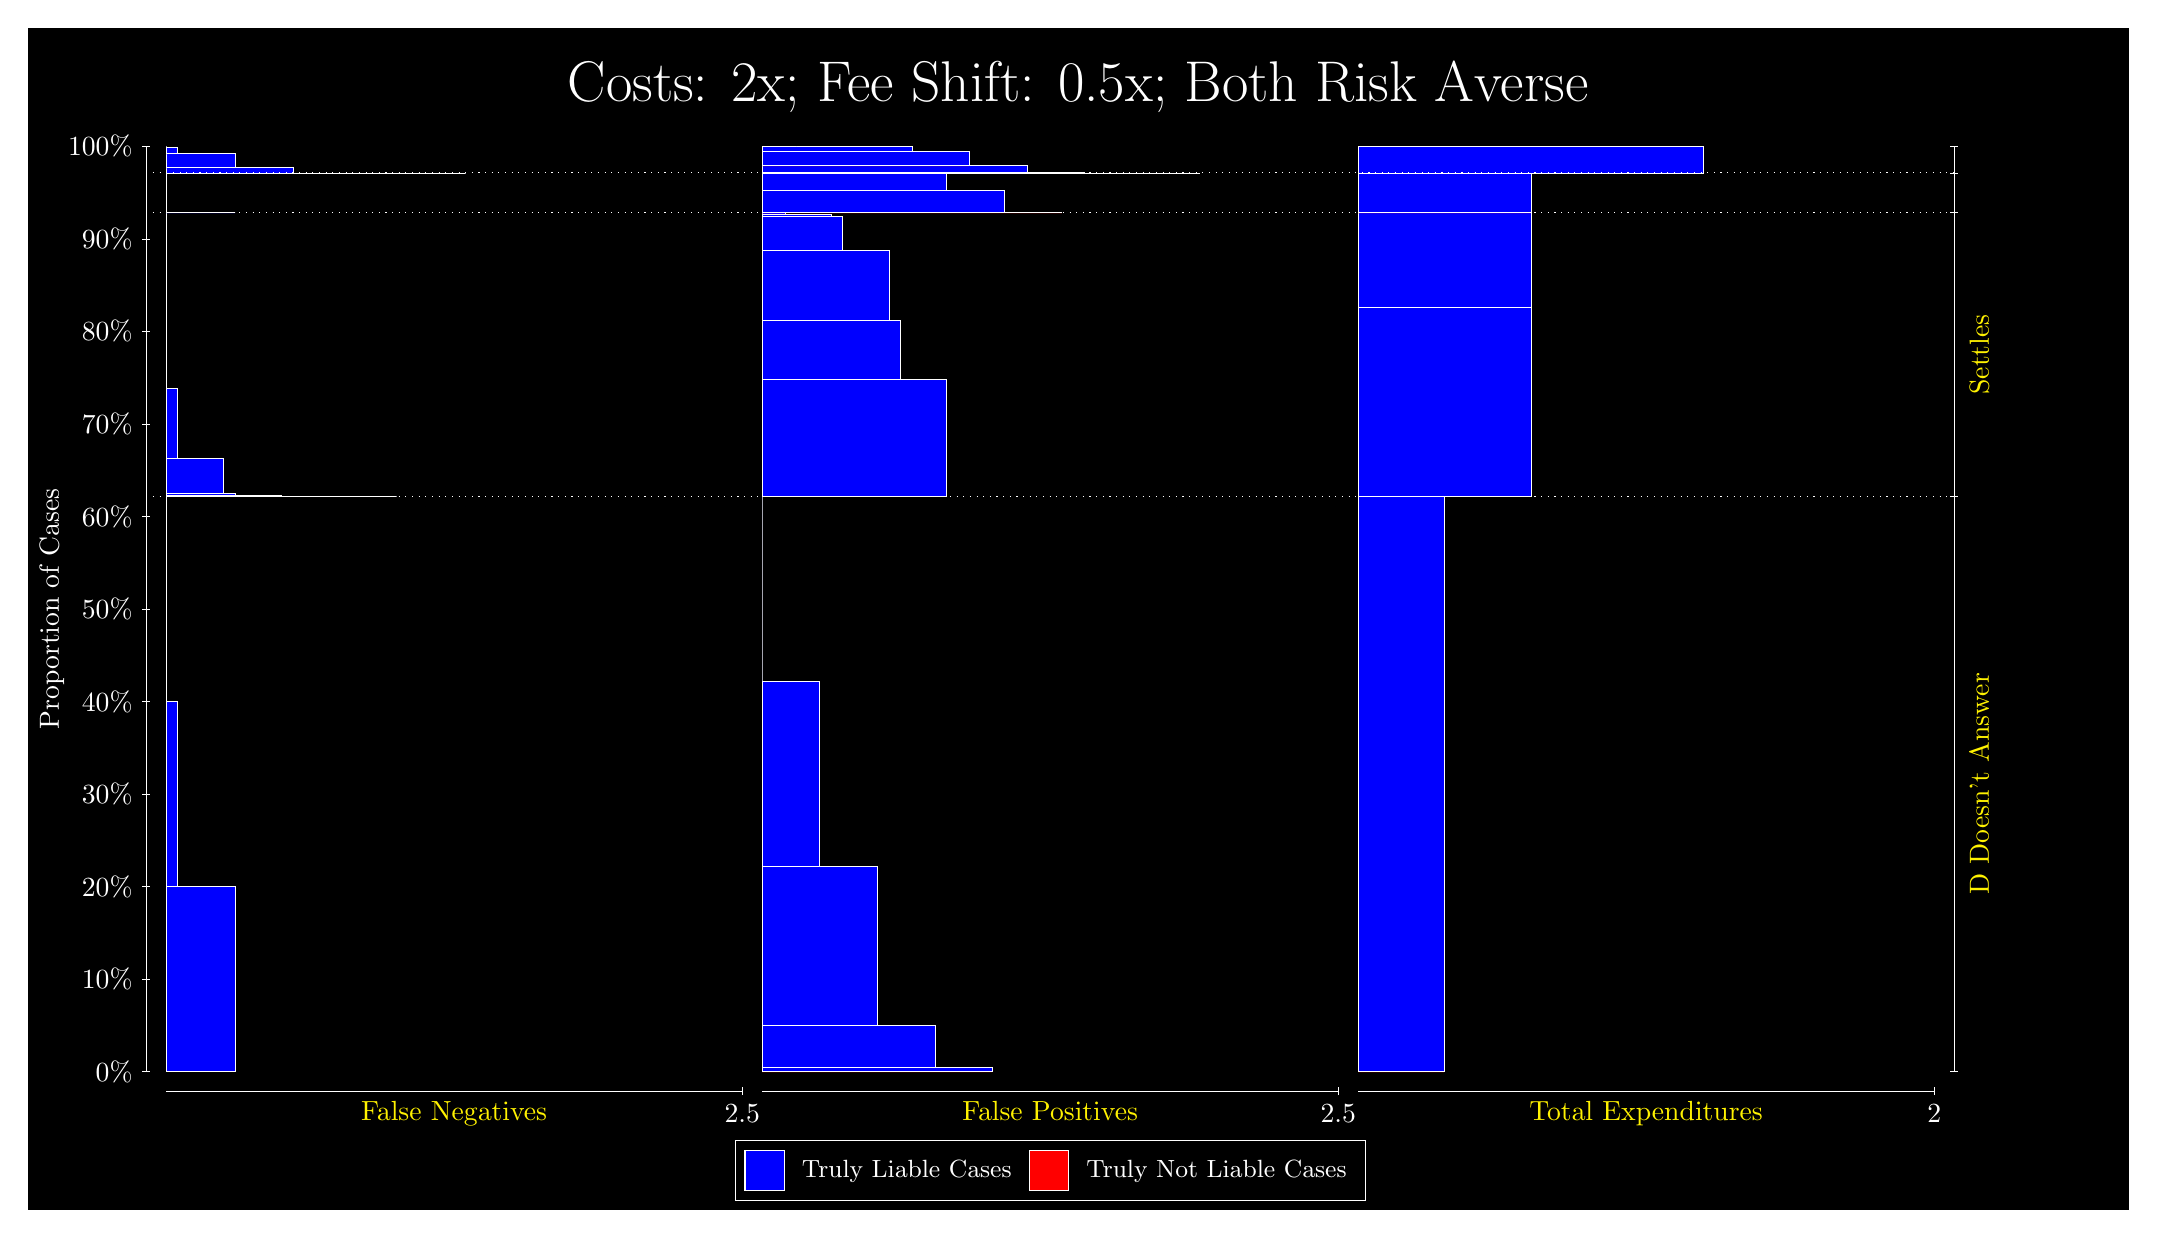
\begin{tikzpicture}
\draw[fill=black] (0,0) rectangle (26.667,15);
\draw[text=white] (0,13.5) rectangle (26.667,15) node[midway] {\huge Costs: 2x; Fee Shift: 0.5x; Both Risk Averse};
\draw[white, very thin] (1.5,1.75) -- (1.5,13.5);
\node[rotate=90, text=white, anchor=center] at (0.3, 7.625) {Proportion of Cases};
\draw[white, very thin] (1.45,1.75) -- (1.55,1.75);
\node[text=white, anchor=east] at (1.45, 1.75) {0\%};
\draw[white, very thin] (1.45,2.925) -- (1.55,2.925);
\node[text=white, anchor=east] at (1.45, 2.925) {10\%};
\draw[white, very thin] (1.45,4.1) -- (1.55,4.1);
\node[text=white, anchor=east] at (1.45, 4.1) {20\%};
\draw[white, very thin] (1.45,5.275) -- (1.55,5.275);
\node[text=white, anchor=east] at (1.45, 5.275) {30\%};
\draw[white, very thin] (1.45,6.45) -- (1.55,6.45);
\node[text=white, anchor=east] at (1.45, 6.45) {40\%};
\draw[white, very thin] (1.45,7.625) -- (1.55,7.625);
\node[text=white, anchor=east] at (1.45, 7.625) {50\%};
\draw[white, very thin] (1.45,8.8) -- (1.55,8.8);
\node[text=white, anchor=east] at (1.45, 8.8) {60\%};
\draw[white, very thin] (1.45,9.975) -- (1.55,9.975);
\node[text=white, anchor=east] at (1.45, 9.975) {70\%};
\draw[white, very thin] (1.45,11.15) -- (1.55,11.15);
\node[text=white, anchor=east] at (1.45, 11.15) {80\%};
\draw[white, very thin] (1.45,12.325) -- (1.55,12.325);
\node[text=white, anchor=east] at (1.45, 12.325) {90\%};
\draw[white, very thin] (1.45,13.5) -- (1.55,13.5);
\node[text=white, anchor=east] at (1.45, 13.5) {100\%};

\draw[white, very thin] (24.457,1.75) -- (24.457,13.5);
\draw[white, very thin] (24.407,1.75) -- (24.507,1.75);
\node[anchor=west] at (24.407, 1.75) {};
\draw[white, very thin] (24.407,9.0547) -- (24.507,9.0547);
\node[anchor=west] at (24.407, 9.0547) {};
\draw[white, very thin] (24.407,12.658) -- (24.507,12.658);
\node[anchor=west] at (24.407, 12.658) {};
\draw[white, very thin] (24.407,13.162) -- (24.507,13.162);
\node[anchor=west] at (24.407, 13.162) {};
\draw[white, very thin] (24.407,13.5) -- (24.507,13.5);
\node[anchor=west] at (24.407, 13.5) {};

\draw[white, very thin, fill=blue] (1.75,1.75) rectangle (2.6283,4.0999);
\draw[white, very thin, fill=blue] (1.75,4.0999) rectangle (1.8964,6.4471);
\draw[white, very thin, fill=red] (1.75,6.4471) rectangle (1.75,6.4471);
\draw[white, very thin, fill=blue] (1.75,6.4471) rectangle (1.75,9.0547);
\draw[white, very thin, fill=blue] (1.75,9.0547) rectangle (4.6775,9.0547);
\draw[white, very thin, fill=blue] (1.75,9.0547) rectangle (4.092,9.0547);
\draw[white, very thin, fill=blue] (1.75,9.0547) rectangle (3.9457,9.0547);
\draw[white, very thin, fill=blue] (1.75,9.0547) rectangle (3.3602,9.0547);
\draw[white, very thin, fill=blue] (1.75,9.0547) rectangle (3.2138,9.0694);
\draw[white, very thin, fill=blue] (1.75,9.0694) rectangle (2.6283,9.0994);
\draw[white, very thin, fill=blue] (1.75,9.0994) rectangle (2.4819,9.5379);
\draw[white, very thin, fill=blue] (1.75,9.5379) rectangle (1.8964,10.427);
\draw[white, very thin, fill=red] (1.75,10.427) rectangle (1.75,10.427);
\draw[white, very thin, fill=blue] (1.75,10.427) rectangle (1.75,12.658);
\draw[white, very thin, fill=blue] (1.75,12.658) rectangle (2.6283,12.658);
\draw[white, very thin, fill=blue] (1.75,12.658) rectangle (1.8964,12.66);
\draw[white, very thin, fill=red] (1.75,12.66) rectangle (1.75,12.66);
\draw[white, very thin, fill=blue] (1.75,12.66) rectangle (1.75,13.162);
\draw[white, very thin, fill=blue] (1.75,13.162) rectangle (5.5558,13.162);
\draw[white, very thin, fill=blue] (1.75,13.162) rectangle (4.8239,13.162);
\draw[white, very thin, fill=blue] (1.75,13.162) rectangle (4.092,13.164);
\draw[white, very thin, fill=blue] (1.75,13.164) rectangle (3.3602,13.229);
\draw[white, very thin, fill=blue] (1.75,13.229) rectangle (2.6283,13.229);
\draw[white, very thin, fill=blue] (1.75,13.229) rectangle (2.6283,13.408);
\draw[white, very thin, fill=blue] (1.75,13.408) rectangle (1.8964,13.408);
\draw[white, very thin, fill=blue] (1.75,13.408) rectangle (1.8964,13.492);
\draw[white, very thin, fill=red] (1.75,13.492) rectangle (1.75,13.492);
\draw[white, very thin, fill=blue] (1.75,13.492) rectangle (1.75,13.5);
\draw[white, very thin, fill=red] (9.3189,1.75) rectangle (12.246,1.75);
\draw[white, very thin, fill=blue] (9.3189,1.75) rectangle (12.246,1.7998);
\draw[white, very thin, fill=blue] (9.3189,1.7998) rectangle (11.515,2.3416);
\draw[white, very thin, fill=blue] (9.3189,2.3416) rectangle (10.783,4.3576);
\draw[white, very thin, fill=blue] (9.3189,4.3576) rectangle (10.051,6.7048);
\draw[white, very thin, fill=blue] (9.3189,6.7048) rectangle (9.3189,9.0547);
\draw[white, very thin, fill=red] (9.3189,9.0547) rectangle (11.661,9.0547);
\draw[white, very thin, fill=blue] (9.3189,9.0547) rectangle (11.661,10.542);
\draw[white, very thin, fill=red] (9.3189,10.542) rectangle (11.075,10.542);
\draw[white, very thin, fill=blue] (9.3189,10.542) rectangle (11.075,11.286);
\draw[white, very thin, fill=blue] (9.3189,11.286) rectangle (10.929,12.175);
\draw[white, very thin, fill=blue] (9.3189,12.175) rectangle (10.344,12.613);
\draw[white, very thin, fill=blue] (9.3189,12.613) rectangle (10.197,12.643);
\draw[white, very thin, fill=blue] (9.3189,12.643) rectangle (9.6116,12.658);
\draw[white, very thin, fill=blue] (9.3189,12.658) rectangle (9.4652,12.658);
\draw[white, very thin, fill=blue] (9.3189,12.658) rectangle (9.3189,12.658);
\draw[white, very thin, fill=red] (9.3189,12.658) rectangle (13.125,12.658);
\draw[white, very thin, fill=blue] (9.3189,12.658) rectangle (13.125,12.666);
\draw[white, very thin, fill=blue] (9.3189,12.666) rectangle (12.393,12.94);
\draw[white, very thin, fill=blue] (9.3189,12.94) rectangle (11.661,13.16);
\draw[white, very thin, fill=blue] (9.3189,13.16) rectangle (10.929,13.162);
\draw[white, very thin, fill=blue] (9.3189,13.162) rectangle (10.197,13.162);
\draw[white, very thin, fill=red] (9.3189,13.162) rectangle (14.881,13.162);
\draw[white, very thin, fill=blue] (9.3189,13.162) rectangle (14.881,13.162);
\draw[white, very thin, fill=red] (9.3189,13.162) rectangle (14.149,13.162);
\draw[white, very thin, fill=blue] (9.3189,13.162) rectangle (14.149,13.163);
\draw[white, very thin, fill=red] (9.3189,13.163) rectangle (13.417,13.163);
\draw[white, very thin, fill=blue] (9.3189,13.163) rectangle (13.417,13.171);
\draw[white, very thin, fill=red] (9.3189,13.171) rectangle (12.686,13.171);
\draw[white, very thin, fill=blue] (9.3189,13.171) rectangle (12.686,13.254);
\draw[white, very thin, fill=red] (9.3189,13.254) rectangle (11.954,13.254);
\draw[white, very thin, fill=blue] (9.3189,13.254) rectangle (11.954,13.434);
\draw[white, very thin, fill=blue] (9.3189,13.434) rectangle (11.222,13.498);
\draw[white, very thin, fill=blue] (9.3189,13.498) rectangle (10.49,13.5);
\draw[white, very thin, fill=blue] (9.3189,13.5) rectangle (9.758,13.5);
\draw[white, very thin, fill=blue] (9.3189,13.5) rectangle (9.3189,13.5);
\draw[white, very thin, fill=red] (16.888,1.75) rectangle (17.986,1.75);
\draw[white, very thin, fill=blue] (16.888,1.75) rectangle (17.986,9.0547);
\draw[white, very thin, fill=red] (16.888,9.0547) rectangle (19.083,9.0547);
\draw[white, very thin, fill=blue] (16.888,9.0547) rectangle (19.083,11.462);
\draw[white, very thin, fill=red] (16.888,11.462) rectangle (19.083,11.462);
\draw[white, very thin, fill=blue] (16.888,11.462) rectangle (19.083,12.658);
\draw[white, very thin, fill=red] (16.888,12.658) rectangle (19.083,12.658);
\draw[white, very thin, fill=blue] (16.888,12.658) rectangle (19.083,13.162);
\draw[white, very thin, fill=red] (16.888,13.162) rectangle (21.279,13.162);
\draw[white, very thin, fill=blue] (16.888,13.162) rectangle (21.279,13.5);
\draw[white, dotted] (1.5,9.0547) -- (24.457,9.0547);
\draw[white, dotted] (1.5,12.658) -- (24.457,12.658);
\draw[white, dotted] (1.5,13.162) -- (24.457,13.162);
\draw[white, very thin] (1.75,1.5) -- (9.0689,1.5);
\node[text=yellow, anchor=north] at (5.4094, 1.5) {False Negatives};
\draw[white, very thin] (9.0689,1.45) -- (9.0689,1.55);
\node[text=white, anchor=north] at (9.0689, 1.45) {2.5};

\draw[white, very thin] (9.3189,1.5) -- (16.638,1.5);
\node[text=yellow, anchor=north] at (12.978, 1.5) {False Positives};
\draw[white, very thin] (16.638,1.45) -- (16.638,1.55);
\node[text=white, anchor=north] at (16.638, 1.45) {2.5};

\draw[white, very thin] (16.888,1.5) -- (24.207,1.5);
\node[text=yellow, anchor=north] at (20.547, 1.5) {Total Expenditures};
\draw[white, very thin] (24.207,1.45) -- (24.207,1.55);
\node[text=white, anchor=north] at (24.207, 1.45) {2};

\node[text=yellow, centered, rotate=90] at (24.777, 5.4023) {D Doesn't Answer};
\node[text=yellow, centered, rotate=90] at (24.777, 10.856) {Settles};



\draw (12.978300999999998,1.5) node[draw=none] (baseCoordinate) {};
\begin{scope}[align=center]
        \matrix[scale=0.5, draw=white, below=0.5cm of baseCoordinate, nodes={draw}, column sep=0.1cm]{
            \node[rectangle, draw, minimum width=0.5cm, minimum height=0.5cm, fill=blue] {}; &
            \node[draw=none, font=\small, text=white] (B) {Truly Liable Cases}; &
            \node[rectangle, draw, minimum width=0.5cm, minimum height=0.5cm, fill=red] {}; &
            \node[draw=none, font=\small, text=white] (B) {Truly Not Liable Cases}; \\
            };
\end{scope}

\end{tikzpicture}
\end{document}